\mode*
%\section[Cronograma]{\iftagged{handout-tufte}{\textcolor{blueun}{\textbf{Cronograma}}}{Cronograma}}
\mode<article|presentation>{%
  \iftagged{handout-tufte}%
  {\section[Cronograma]{\textbf{\textcolor{blueun}{Cronograma}}}}%
  {\section[Cronograma]{Cronograma}}
}%
\label{sec:cronograma}

\untagged{handout-tufte}{En la secci\'on anterior, cada paso tiene un nombre resaltado en negrita, a estos 14 nombres se le denominar\'an Actividades en la tabla a mostrada a continuaci\'on (\tablename  \ref{tab:crono} y \ref{tab:crono2}.). }La tabla del cronograma muestra también como se piensa ejecutar la metodolog\'ia propuesta anterior.\par

\mode<presentation>{
  \begin{frame}[label=cronograma]
    \transduration{2}
    \frametitle{Cuando se espera resolver?}
    \begin{center}
      \LARGE \textbf{\textcolor{blueun}{Cronograma}}
    \end{center}      
  \end{frame}
  \begin{frame}[label=simulacion_cronograma]
    \transduration<1>{2}
    \transduration<2-3>{4}
    \transduration<4>{2}
    \frametitle{Cronograma de la Metodolog\'ia}
    \begin{center}
      \only<1>{
        \textbf{\textcolor{blueun}{Evoluci\'on del Framework}}

        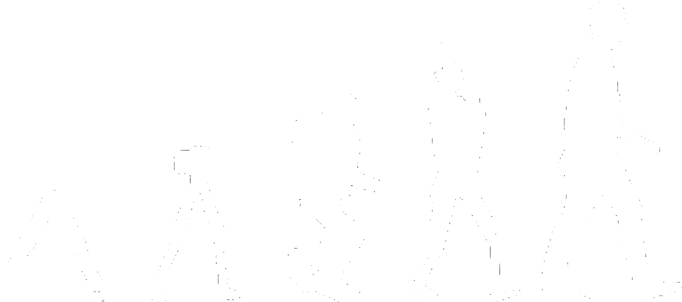
\includegraphics[height=2.0cm]{../images/EvolutionFramework_0.png}

        \animategraphics[height=3.5cm,autoresume,autoplay]{3}{../images/Cronograma_}{0}{5}
      }
      \only<2>{
        \textbf{\textcolor{blueun}{Evoluci\'on del Framework}}

        \animategraphics[height=2.0cm,autoresume,autoplay]{1.5}{../images/EvolutionFramework_}{0}{4}
        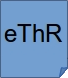
\includegraphics[height=0.6cm]{../images/TechReportLogo.png}

        \animategraphics[height=3.5cm,autoresume,autoplay]{3}{../images/Cronograma_}{6}{17}
      }
      \only<3>{
        \textbf{\textcolor{blueun}{Evoluci\'on del Framework}}

        \animategraphics[height=2.0cm,autoresume,autoplay]{1.5}{../images/EvolutionFramework_}{6}{12}
        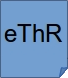
\includegraphics[height=0.6cm]{../images/TechReportLogo.png}

        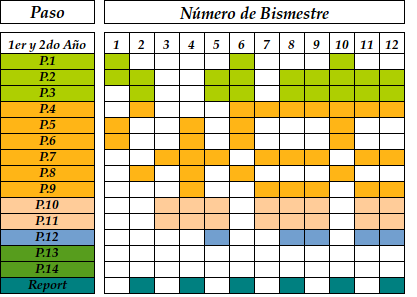
\includegraphics[height=3.5cm]{../images/Cronograma_17.png}
        \animategraphics[height=3.5cm,autoresume,autoplay]{3}{../images/Cronograma_}{18}{29}
      }
      \only<4>{
        \textbf{\textcolor{blueun}{Evoluci\'on del Framework}}

        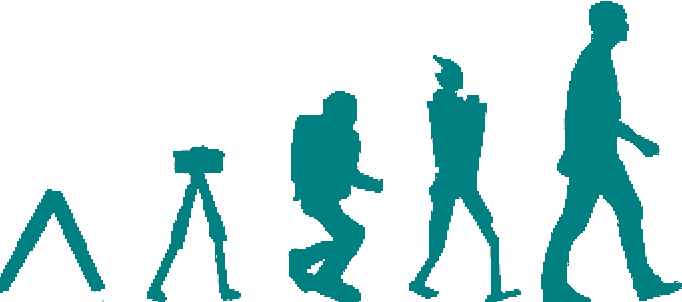
\includegraphics[height=2.0cm]{../images/EvolutionFramework_10.png}
        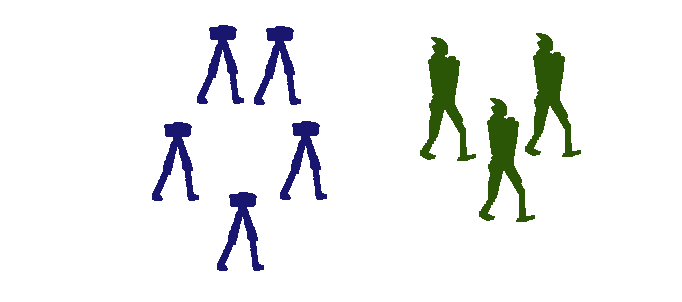
\includegraphics[height=2.0cm]{../images/EvolutionFramework_12.png}
        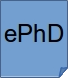
\includegraphics[height=0.6cm]{../images/PhDLogo.png}

        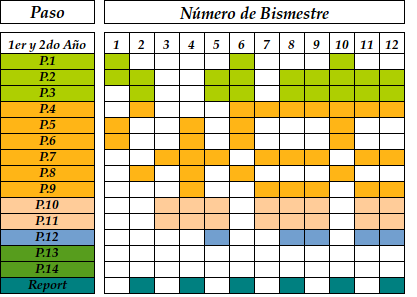
\includegraphics[height=3.5cm]{../images/Cronograma_17.png}
        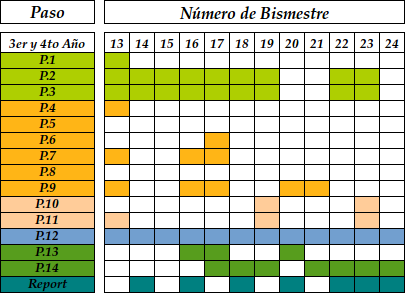
\includegraphics[height=3.5cm]{../images/Cronograma_29.png}
      }
    \end{center}
  \end{frame}
}
\iftagged{handout-tufte}{
  \begin{figure}
    \centering
    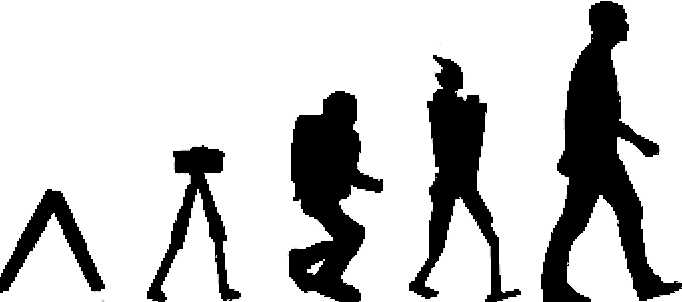
\includegraphics[width=2.0cm]{../images/EvolutionFramework_5.png}
    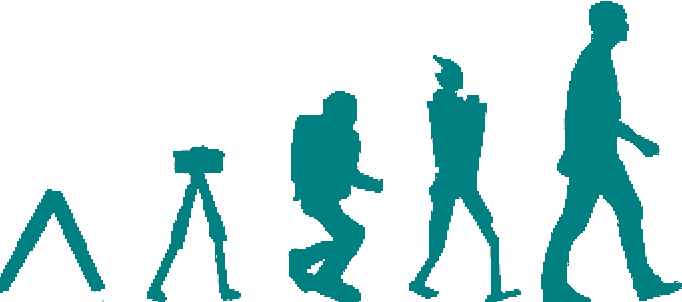
\includegraphics[width=2.0cm]{../images/EvolutionFramework_10.png}
    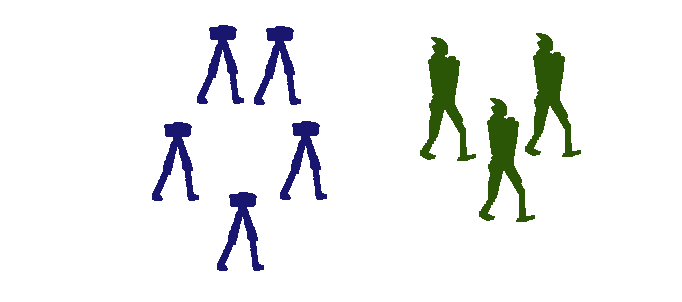
\includegraphics[width=2.0cm]{../images/EvolutionFramework_12.png}
    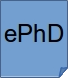
\includegraphics[width=0.6cm]{../images/PhDLogo.png}\\
    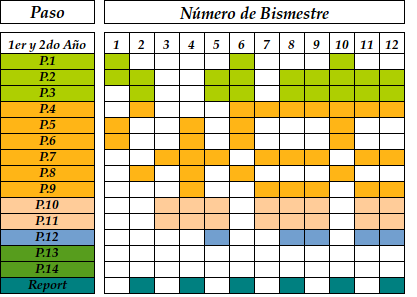
\includegraphics[width=3.5cm]{../images/Cronograma_17.png}
    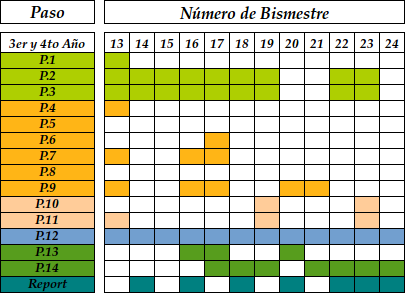
\includegraphics[width=3.5cm]{../images/Cronograma_29.png}    
    \caption{Evoluci\'on del Framework}
    \label{fig:cronoMeto}
  \end{figure}
}{
  \begin{table}[!htb]
    \centering
    \newcolumntype{G}{>{\columncolor[gray]{0.0}}c}
    \newcommand{\Bk}{\multicolumn{1}{G}{ }}
    \begin{tabular}{|p{3.0cm}||c|c|c|c|c|c|c|c|c|c|c|c|}\hline
      Actividades&\multicolumn{12}{|c|}{Bimestre}\\\hline\hline
      1er y  2do A\~no&1&2 &3  &4  &5  &6  &7  &8  &9  &10 &11 &12 \\\hline
      \textbf{P} 1. &\Bk&   &   &   &   &\Bk&   &   &   &\Bk&   &   \\\hline
      \textbf{P} 2. &\Bk&\Bk&   &   &\Bk&\Bk&   &\Bk&\Bk&\Bk&\Bk&\Bk\\\hline
      \textbf{P} 3. &   &\Bk&   &   &\Bk&\Bk&   &\Bk&\Bk&\Bk&\Bk&\Bk\\\hline
      \textbf{P} 4. &   &\Bk&   &   &   &\Bk&\Bk&\Bk&\Bk&\Bk&\Bk&\Bk\\\hline
      \textbf{P} 5. &\Bk&   &   &\Bk&   &\Bk&   &   &   &\Bk&   &   \\\hline
      \textbf{P} 6. &\Bk&   &   &\Bk&   &\Bk&   &   &   &\Bk&   &   \\\hline
      \textbf{P} 7. &   &   &\Bk&\Bk&\Bk&   &\Bk&\Bk&\Bk&   &\Bk&\Bk\\\hline
      \textbf{P} 8. &   &\Bk&   &\Bk&   &\Bk&   &   &   &\Bk&   &   \\\hline
      \textbf{P} 9. &   &   &   &\Bk&   &   &\Bk&\Bk&\Bk&   &\Bk&\Bk\\\hline
      \textbf{P} 10.&   &   &\Bk&\Bk&\Bk&   &\Bk&\Bk&\Bk&   &\Bk&\Bk\\\hline
      \textbf{P} 11.&   &   &\Bk&\Bk&\Bk&   &\Bk&\Bk&\Bk&   &\Bk&\Bk\\\hline
      \textbf{P} 12.&   &   &   &   &\Bk&   &   &\Bk&\Bk&   &\Bk&\Bk\\\hline
      \textbf{P} 13.&   &   &   &   &   &   &   &   &   &   &   &   \\\hline
      \textbf{P} 14.&   &   &   &   &   &   &   &   &   &   &   &   \\\hline
      Escribir Doc &   &\Bk&   &\Bk&   &\Bk&   &\Bk&   &\Bk&   &\Bk\\\hline    
    \end{tabular}
    \caption{Cronograma de investigaci\'on de los primeros dos a\~nos}
    \label{tab:crono}
  \end{table}
  \begin{table}[!htb]
    \centering
    \newcolumntype{G}{>{\columncolor[gray]{0.0}}c}
    \newcommand{\Bk}{\multicolumn{1}{|G|}{ }}
    \begin{tabular}{|p{3.0cm}||c|c|c|c|c|c|c|c|c|c|c|c|}\hline
      Actividades&\multicolumn{12}{|c|}{Bimestre}\\\hline\hline
      % 3er y  4to A\~no &13 &14 &15 &16 &17 &18 &19 &20 &21 &22 &23 &24 \\\hline
      1er y  2do A\~no&1&2 &3  &4  &5  &6  &7  &8  &9  &10 &11 &12 \\\hline
      \textbf{P} 1. &\Bk&   &   &   &   &   &   &   &   &   &   &   \\\hline
      \textbf{P} 2. &\Bk&\Bk&\Bk&\Bk&\Bk&\Bk&\Bk&   &   &\Bk&\Bk&   \\\hline
      \textbf{P} 3. &\Bk&\Bk&\Bk&\Bk&\Bk&\Bk&\Bk&   &   &\Bk&\Bk&   \\\hline
      \textbf{P} 4. &\Bk&   &   &   &   &   &   &   &   &   &   &   \\\hline
      \textbf{P} 5. &   &   &   &   &   &   &   &   &   &   &   &   \\\hline
      \textbf{P} 6. &   &   &   &   &\Bk&   &   &   &   &   &   &   \\\hline
      \textbf{P} 7. &\Bk&   &   &\Bk&\Bk&   &   &   &   &   &   &   \\\hline
      \textbf{P} 8. &   &   &   &   &   &   &   &   &   &   &   &   \\\hline
      \textbf{P} 9. &\Bk&   &   &\Bk&\Bk&   &   &\Bk&\Bk&   &   &   \\\hline
      \textbf{P} 10.&   &   &   &   &   &   &\Bk&   &   &   &\Bk&   \\\hline
      \textbf{P} 11.&\Bk&   &   &   &   &   &\Bk&   &   &   &\Bk&   \\\hline
      \textbf{P} 12.&\Bk&\Bk&\Bk&\Bk&\Bk&\Bk&\Bk&\Bk&\Bk&\Bk&\Bk&\Bk\\\hline
      \textbf{P} 13.&   &   &   &\Bk&\Bk&   &   &\Bk&   &   &   &   \\\hline
      \textbf{P} 14.&   &   &   &   &\Bk&\Bk&\Bk&   &\Bk&\Bk&\Bk&\Bk\\\hline
      Escribir Doc &   &\Bk&   &\Bk&   &\Bk&   &\Bk&   &\Bk&\Bk&\Bk\\\hline    
    \end{tabular}
    \caption{Cronograma de investigaci\'on de los dos \'ultimos a\~nos}
    \label{tab:crono2}
  \end{table}
}
